\documentclass[12pt,a4paper]{article}
%-------------------------------------------
%---Packages--------------------------------
%-------------------------------------------
\usepackage[utf8]{inputenc}
%\usepackage[T1]{fontenc}
%\usepackage{txfonts}
\usepackage{amsmath}
\usepackage{amsthm}
\usepackage{amsfonts}
\usepackage{array}
\usepackage{amssymb}
\usepackage{blindtext}
\usepackage{caption}
\usepackage{color}
\usepackage{csquotes}	    %
\usepackage{enumitem}	    %pour mieux bosser avec les listes. ajoute option label
\usepackage[yyyymmdd]{datetime}        %pour définir date custom
\usepackage{etaremune}
\usepackage{environ}
\usepackage{fancybox}
\usepackage{fancyhdr} 	    % Custom headers and footers
\usepackage{fancyref}
%\usepackage{float}
\usepackage{floatrow}       %float and floatrow can't be together...
\usepackage{gensymb}
\usepackage{graphicx}
\usepackage[colorlinks=true, linkcolor=purple, citecolor=cyan]{hyperref}
\usepackage{footnotebackref}
\usepackage{lipsum}
\usepackage{mathtools}
\usepackage{multicol}	    %gérer plusieurs colonnes
\usepackage{setspace}
\usepackage{subcaption}
\usepackage{todonotes}	    %Bonne gestion des TODOs
%TODO commenté pour tester l'utilité... à voir% \usepackage[tc]{titlepic}      %Permet de mettre une image en page de garde
\usepackage{tikz}	    % Pour outil de dessin puissant
\usepackage{ulem}	    %underline sur plusieurs lignes (avec \uline{})
\usepackage{vmargin} 	    %gestion des marges, avec dans l'ordre : gauche, haut, droit, bas, en-tête, entre en-tête et texte, bas de page, hauteur entre bas de page et texte
\usepackage{wrapfig}
\usepackage{xcolor}
\usepackage{xparse}                    %Pour utiliser NewDocumentCommand et des arguments 'mmooo'
%\usepackage{fullpage} 	    %supprime toutes les marges allouées aux notes, aussi en haut et en bas

%\ExplSyntaxOn
\pagestyle{fancyplain}	    %Makes all pages in the document conform to the custom headers and footers

%-------------------------------------------
%---Document Commands-----------------------
%---------------------------{----------------
\NewDocumentCommand{\framecolorbox}{oommm}
 {% #1 = width (optional)
  % #2 = inner alignment (optional)
  % #3 = frame color
  % #4 = background color
  % #5 = text
  \IfValueTF{#1}%
   {\IfValueTF{#2}%
    {\fcolorbox{#3}{#4}{\makebox[#1][#2]{#5}}}%
    {\fcolorbox{#3}{#4}{\makebox[#1]{#5}}}%
   }%
   {\fcolorbox{#3}{#4}{#5}}%
 }%
%------------------------------------------------
%------------------ENGLISH----------------------
%----------------------------------------------

\NewDocumentCommand{\epflTitle}{mO{Olivier Cloux}O{\today}O{Notes de Cours en}D<>{../../Common}}%Arguments : Matière, Auteur, Date, Titre du doc
{
\begin{titlepage}
    \vspace*{\fill}
    \begin{center}
        \normalfont \normalsize
        \textsc{Ecole Polytechnique Fédérale de Lausanne} \\ [25pt] % Your university, school and/or department name(s)
        \textsc{#4} %Titre du doc
        \\ [0.4 pt]
        \horrule{0.5pt} \\[0.4cm] % Thin top horizontal rule
        \huge #1 \\ % Matière
        \horrule{2pt} \\[0.5cm] % Thick bottom horizontal rule
        
\includegraphics[width=8cm]{#5/EPFL_logo}
        ~\\[0.5 cm]
        \small\textsc{#2}\\[0.4cm]
        \small\textsc{#3}\\
        ~\\
        ~\\
        
\includegraphics[scale=0.5]{#5/creativeCommons}
    \end{center}
    \vspace*{\fill}
\end{titlepage}
}


%-------------------------------------------
%-------------MATH NEW COMMANDS-------------
%-------------------------------------------
\newcommand{\somme}[2]{\ensuremath{\sum\limits_{#2}^{#1}}}
\newcommand{\produit}[2]{\ensuremath{\prod\limits_{#2}^{#1}}}
\newcommand{\limite}{\lim\limits_}
\newcommand{\llimite}[3]{\limite{\substack{#1 \\ #2}}\left(#3\right)}	%limites à deux condiitons
\newcommand{\et}{\mbox{ et }}
\newcommand{\deriv}[1]{\ensuremath{\, \mathrm d #1}}	%sigle dx, dt,dy... des dérivées/intégrales
%\newcommand{\fx}{\ensuremath{f'(\textbf{x}_0 + h}}
\newcommand{\ninf}{\ensuremath{n \to \infty}}	       %pour les limites : n tend vers l'infini
\newcommand{\xinf}{\ensuremath{x \to \infty}}	       %pour les limites : x tend vers l'infini
\newcommand{\infint}{\ensuremath{\int_{-\infty}^{\infty}}}
\newcommand{\xo}{\ensuremath{x \to 0}}									%x to 0
\newcommand{\no}{\ensuremath{n \to 0}}									%n zéro
\newcommand{\xx}{\ensuremath{x \to x}}									%x to x
\newcommand{\Xo}{\ensuremath{x_0}}										%x zéro
\newcommand{\X}{\ensuremath{\mathbf{X}} }
\newcommand{\A}{\ensuremath{\mathbf{A}} }
\newcommand{\R}{\ensuremath{\mathbb{R}} }								%ensemble de R
\newcommand{\rn}{\ensuremath{\mathbb{R}^n} } 							%ensemble de R de taille n
\newcommand{\Rm}{\ensuremath{\mathbb{R}^m} }  							%ensemble de R de taille m
\newcommand{\C}{\ensuremath{\mathbb{C}} }
\newcommand{\N}{\ensuremath{\mathbb{N}} }
\newcommand{\Z}{\ensuremath{\mathbb{Z}} }
\newcommand{\Q}{\ensuremath{\mathbb{Q}} }
\newcommand{\rtor}{\ensuremath{\R \to \R} }
\newcommand{\pour}{\mbox{ pour }}
\newcommand{\coss}[1]{\ensuremath{\cos\(#1\)}}						%cosinus avec des parenthèses de bonne taille (genre frac)
\newcommand{\sinn}[1]{\ensuremath{\sin\(#1\)}}					%sinus avec des parentèses de bonne taille (genre frac)
\newcommand{\txtfrac}[2]{\ensuremath{\frac{\text{#1}}{\text{#2}}}}		%Fractions composées de texte
\newcommand{\evalfrac}[3]{\ensuremath{\left.\frac{#1}{#2}\right|_{#3}}}
\renewcommand{\(}{\left(}												%Parenthèse gauche de taille adaptive
\renewcommand{\)}{\right)}
\newcommand{\longeq}{=\joinrel=}												%Parenthèse droite de taille adaptive


%-------------------------------------------------------
%------------------MISC NEW COMMANDS--------------------
%-------------------------------------------------------
\newcommand{\degre}{\ensuremath{^\circ}}
%\newdateformat{\eudate}{\THEYEAR-\twodigit{\THEMONTH}-\twodigit{\THEDAY}}



%-------------------------------------------------------
%------------------TEXT NEW COMMANDS--------------------
%-------------------------------------------------------
\newcommand{\ts}{\textsuperscript}
\newcommand{\evid}[1]{\textbf{\uline{#1}}}        %mise en évidence (gras + souligné)



%\newcommand{\Exemple}{\underline{Exemple}}
\newcommand{\Theoreme}{\underline{Théorème}}
\newcommand{\Remarque}{\underline{Remarque}}
\newcommand{\Definition}{\underline{Définition} }
\newcommand{\skinf}{\sum^{\infty}_{k=0}}
\newcommand{\combi}[2]{\ensuremath{\begin{pmatrix} #1 \\ #2 \end{pmatrix}}}	%combinaison parmi 1 de 2
\newcommand{\intx}[3]{\ensuremath{\int_{#1}^{#2} #3 \deriv{x}}}				%intégrale dx
\newcommand{\intt}[3]{\ensuremath{\int_{#1}^{#2} #3 \deriv{t}}}				%intégrale dy
\newcommand{\misenforme}{\begin{center} Mis en forme jusqu'ici\\ \line(1,0){400}\\ normalement juste, mais à améliorer depuis ici\end{center}}	%raccourci pour mise en forme
\newcommand*\circled[1]{\tikz[baseline=(char.base)]{
            \node[shape=circle,draw,inner sep=1pt] (char) {#1};}}			%pour entourer un chiffre
\newcommand{\horrule}[1]{\rule{\linewidth}{#1}} 				% Create horizontal rule command with 1 argument of height

\theoremstyle{definition}
\newtheorem{exemp}{Exemple}
\newtheorem{examp}{Example}


%-------------------------------------------
%---Environments----------------------------
%-------------------------------------------
\NewEnviron{boite}[1][0.9]{%
	\begin{center}
		\framecolorbox{red}{white}{%
			\begin{minipage}{#1\textwidth}
 	 			\BODY
			\end{minipage}
		}
	\end{center}
}
\NewEnviron{blackbox}[1][0.9]{%
	\begin{center}
		\framecolorbox{black}{white}{%
			\begin{minipage}{#1\textwidth}
 	 			\BODY
			\end{minipage}
		}
	\end{center}
}
\NewEnviron{exemple}[1][0.8]{%
    \begin{center}
        \framecolorbox{white}{gray!20}{%
            \begin{minipage}{#1\textwidth}
                \begin{exemp}
                    \BODY
                \end{exemp}
            \end{minipage}
        }
    \end{center}
}
\NewEnviron{suiteExemple}[1][0.8]{%
    \begin{center}
        \framecolorbox{white}{gray!20}{%
            \begin{minipage}{#1\textwidth}
                \BODY
            \end{minipage}
        }
    \end{center}
}
\NewEnviron{colExemple}[1][0.8]{%
    \begin{center}
        \framecolorbox{white}{gray!20}{%
            \begin{minipage}{#1\columnwidth}
                \begin{exemp}
                    \BODY
                \end{exemp}
            \end{minipage}
        }
    \end{center}
}
\NewEnviron{example}[1][0.8]{%
    \begin{center}
        \framecolorbox{white}{gray!20}{%
            \begin{minipage}{#1\textwidth}
                \begin{examp}
                    \BODY
                \end{examp}
            \end{minipage}
	}
    \end{center}
}
\NewEnviron{systeq}[1][l]{
			\begin{center}
				$\left\{\begin{array}{#1}
					\BODY
				\end{array}\right.$
			\end{center}
 }





%-------------------------------------------
%---General settings-----------------------
%-------------------------------------------
\renewcommand{\headrulewidth}{1pt}										%ligne au haut de chaque page
\renewcommand{\footrulewidth}{1pt}										%ligne au pied de chaque page
\setstretch{1.6}
\author{Olivier Cloux}

\usepackage[tc]{titlepic}
\usepackage{graphicx}
\usepackage{blindtext}
\newcommand{\E}{\ensuremath{\mathrm{E}}}
%\setcounter{section}{-1}
\newcommand{\indep}{\rotatebox[origin=c]{90}{$\models$}}
%%%%%%%%%%%%%%%%%%%%%%%%%%%%%%%%%%%%%%%%%%
%TODO : Supprimer quand plus de todo %%%%%
\marginparwidth = 75pt
\textwidth = 400pt
%%%%%%%%%%%%%%%%%%%%%%%%%%%%%%%%%%%%%%%%%%%%
\begin{document}
\setstretch{0.9}
\epflTitle{Probability and Statistics}[Olivier Cloux][Spring 2016][Personal summary in]
\newpage
\tableofcontents

\section{Week 1}
Concerns slides 1 to 60. Combinatorics and elements of probability.
\subsection{Theorems and definitions}
\evid{Definition 1.} A \textcolor{red}{set} $A$ is an \textit{unordered} collection of objects $x_1,...,x_n,...$.:
\begin{equation}
    A = \{x,1,...,x_n,...\}
\end{equation}
 $x \in A$ means '$x$ is an element of $A$'. All possible objects in a given context is the \textcolor{red}{universe} $\Omega$. An \textbf{ordered set} is written $A = (1,2,...)$, making $\{1,2\} \neq \{2,1\}$
 
\evid{Definition 2.} A \textcolor{red}{subset} A of B means that an element in A must be in B too. 

\evid{Definition 5.} A \textcolor{red}{partition} of $\Omega$ is a collection of non-empty subsets $A_1 \cup \ldots \cup A_n$ in $\Omega$, such that they are \textbf{exhaustive} (their union makes all $\Omega$) and \textbf{disjoint} (they don't overlap)

\subsubsection*{Reminders in Combinatoric :} Two basic principles : 
\begin{itemize}
    \item \textcolor{red}{multiplication} : $m$ hats and $n$ scarves give me $m\times n$ different combinations of hats and scarves. Mathematically : 
            \begin{equation}
                |A_1 \times \ldots \times A_k| = |A_1| \times \ldots \times |A_k|
            \end{equation}
    \item \textcolor{red}{addition} : $m$ blue hats and $n$ red hats give me $m+n$ hats. Mathematically, if the $A_j$ are disjoints :
            \begin{equation}
                |A_1 \cup \ldots \cup A_k| = |A_1| + \ldots + |A_k|
            \end{equation}
\end{itemize}

\evid{Definition 10.} A \textcolor{red}{permutation} of $n$ distinct objects is an ordered set of those objects

\evid{Theorem 11.} Given $n$ distinct objects, the number of different \textcolor{red}{permutations} (\uline{without repetition}) of length $r \leq n$ is 
\begin{equation}
    n(n-1)(n-1)\ldots(n-r+1) = \frac{n!}{(n-r)!}
    \label{equ:permutations}
\end{equation}
Thus, $n!$ permutations of length $n$.

\evid{Theorem 12.} Given $n = \sum_{i=1}^{r}n_i$ objects of $r$ different types, where $n_i$ is the number of objects of type $i$ (indistinguishable from one another), the number of permutations (\uline{without repetition}) of the $n$ objects is :
\begin{equation}
    \frac{n!}{n_1!n_2!\ldots n_r!}
\end{equation}

\evid{Definition 14.} Let $n_1,...,n_r$ be integers in $0,1,...,n$, having total $n_1+\ldots+n_r = n$. Then 
\begin{equation}
    \combi{n}{n_1,n_2,...,n_r} = \frac{n!}{n_1!n_2!\ldots n_r!}
\end{equation}
is called the \textcolor{red}{multinomial coefficient}. The most common case arises when $r = 2$ :
\begin{equation}
    \combi{n}{k} = \frac{n!}{k!(n-k)!} = C_n^k
\end{equation}
It is called a \textcolor{red}{binomial coefficient}n!

\evid{Theorem 15.} \textcolor{red}{Non ordered selection :} The number of ways of choosing a set of $r$ objects from a set of $n$ distinct objects without repetition is $\combi{n}{r}$

\evid{Theorem 16.} The number of ways of distributing $n$ distinct objects into $r$distinct groups of size $n_1,\ldots,n_r$ where $n_1+\ldots+n_r = n$ is $\frac{n!}{n_1!n_2!\ldots n_r!}$

\evid{Theorem 21} A \textcolor{red}{geometric series} is of the form $a, a\theta, a\theta^2,...$ we have :
\begin{equation}
    \sum_{i=0}^{n} a\theta^i = 
    \left\{\begin{array}{ll}
        a\frac{1-\theta^{n+1}}{1-\theta} & \theta \neq 1\\
        a(n+1) & \theta = 1
    \end{array}\right.
\end{equation}
The \textcolor{red}{exponential series} 
\begin{equation}
    \exp(x) = \sum_{i=0}^{\infty} \frac{x^n}{n!}
\end{equation}
converges absolutely for all $x \in \C$

\subsubsection*{Probability spaces}
\evid{Definition 22.} A \textcolor{red}{random experiment} is an experiment whose result is (or can be defined as) random.

\evid{Definition 28.} A \textcolor{red}{probability space} $(\Omega, F, P)$ is a mathematical object associated with a random experiment, comprising :
\begin{itemize}
    \item A set $\Omega$, the \textbf{sample space (universe)} which contains all the possible \textbf{outcomes} $\omega$ of the experiment.
    \item a collection $F$ of subsets of $\Omega$. They are called \textbf{events}, and $F$ is called the \textbf{event space}.
    \item a function $P : F \to [0,1]$ called a \textbf{probability distribution}, which associates a probability $P(A) \in [0,1]$ to each $A \in F$
\end{itemize}
The sample space is the space composed of elements representing all the possible results of a random experiment. Each element $\omega \in \Omega$ is associated with a different result.

\subsection{Examples}
\evid{Three dice problem} We throw 3 dice. Consider the events : ``total is 9'' and ``total is 10''. First happens with (6,2,1)(5,3,1)(5,2,2)(4,4,1)(4,3,2)(3,3,3) when second happens with (6,3,1)(6,2,2)(5,4,1)(5,3,2)(4,4,2)(4,3,3). Both times 6 possible events, so equi-probable. NO ! as each combination has not the same probability to happen. (3,3,3) has ``weight'' 1 when (4,3,2) has ``weight'' 3!. Thus, the probabilities are different.
\subsection{Exercises}


%%%%%%%%%%%%%%%%%%%%%%%%%%%%%%%%%%%%%%%%%%
%%%%%%%%%%%%%%%%%%%%%%%%%%%%%%%%%%%%%%%%%%
%%%%%%%%%%%%%%%%%%%%%%%%%%%%%%%%%%%%%%%%%%


\section{Week 2}
Concerns slides 62 to 86. Probability spaces, conditional probability, independence.
\subsection{Theorems and definitions}
\evid{Definition 40} Let $A,b$ be events of the probability space $(\Omega, F, P)$, such that $P(B) > 0$. Then the \textbf{conditional probability of $A$ given $B$} is 
\begin{equation}
    P(A|B) = \frac{p(A \cap B)}{P(B)}
    \label{equ: conditional probability}
\end{equation}
\evid{Theorem 43} \textbf{Law of total probability :} Let $\{B_i\}^\infty_{i=1}$ be pairwise disjoints events of the probability space $(\Omega, F, O)$, and let $A$ be an event satisfying $A \subset \bigcup_{i=1}^\infty B_i$. Then :
\begin{equation}
    P(A) = \sum_{i=1}^{\infty} P(A\cap B_i) = \sum_{i=1}^{\infty}P(A|B_i)P(B_i)
\end{equation}
\evid{Theorem 44} \textbf{Bayes' theorem :} Suppose that the conditions above are satisfied, and that $P(A) > 0$. Then 
\begin{equation}
    P(B_j|A) = \frac{P(A|B_j)P(B_j)}{\sum_{i=1}^{\infty}P(A|B_i)P(B_i)} \quad j\in \N
\end{equation}
\evid{Theorem 46} \textbf{Multiple conditioning : Prediction decomposition} Let $A_1,...,A_n$ be events in a probability space. Then :
\begin{equation}
    \begin{array}{rcl}
        P(A_1 \cap A_2) & = & P(A_2|A_1)P(A_1)\\
        P(A_1 \cap A_2 \cap A_3 & = & P(A_3|A_1\cap A_2)P(A_2|A_1)P(A_1)\\
        &\vdots&\\
        P(A_1\cap \ldots \cap A_n) & = & \prod_{i=2}^{n} P(A_i|A_1 \cap \ldots \cap A_{i-1} \times P(A_1)
    \end{array}
\end{equation}
\subsection{Examples}
\evid{Example 41.} \uline{Q :} We roll two far dice, one red and one green. Let $A$ and $B$ be the events ``the total exceeds 8'' and ``we get 6 on the red die''. If we know that B has occurred, how does P(A) change ?\\
\uline{A :} $P(A) = \frac{1+2+3+4}{36} = \frac{5}{18}$ while $P(B) = \frac{1}{6}$. By definition of conditional probability :
\[P(A|B) = \frac{P(A\cap B)}{P(B)} = \frac{4/36}{1/6} = \frac{2}{3}\]

\subsubsection*{Independence}

\evid{Definition 49.} Let $(\Omega, F, P)$ be a probability space. Two events $A,b \in F$ are \textcolor{red}{independent} (we write $A \indep B$) iff
\begin{equation}
    P(A \cap B) = P(A)P(B)
\end{equation}

\evid{Definition 51.} \textcolor{red}{Type of independence :} 
\begin{enumerate}
    \item $A_1,...,A_n$  \textbf{mutually independent} if for al sets of indices $F \subset \{1,...,n\},$
            \[P\(\bigcap_{i\in F} A_i \) = \prod_{i\in F} P(A_i)\]
    \item $A_1,...,A_n$ are \textbf{pairwise independent} if
            \[P(A_i \cap A_j) = P(A_i)P(A_j),\quad 1 \leq i < j \leq n\]
    \item $A_1,...A_n$ are \textbf{conditionally independent given $B$} if for all sets of indices $F \subset \{1,...,n\},$
            \[P\(\bigcap_{i\in F} A_i|B \) = \prod_{i\in F} P(A_i|B)\]
\end{enumerate}
\evid{Example 45.} \uline{Q :} You suspect that the man in front of you at the security check at the airport is a terrorist. Knowing that one person out of $10^6$ is a terrorist, and that a terrorist is detected by the security check with a probability of 0.9999, but that the alarm goes off when an ordinary person goes through with a probability of $10^{-5}$ , what is the probability that he is a terrorist, given that the alarm goes off when he passes through security?\\
\uline{A :} Let $A$ ant $T$ respectively denote the events ``the alarm sounds'' and ``he is a terrorist''. Then we seek
\[P(T|A) = \frac{P(A|T)P(T)}{P(A|T)P(T) + P(A|T^c)(T^c)} = \frac{0.999 \times 10^{-6}}{0.9999\times 10^{-6} + 10^{-5} \times (1-10^{-6})} = 0.0909\]
\subsection{Exercises}

%%%%%%%%%%%%%%%%%%%%%%%%%%%%%%%%%%%%%%%%%%
%%%%%%%%%%%%%%%%%%%%%%%%%%%%%%%%%%%%%%%%%%
%%%%%%%%%%%%%%%%%%%%%%%%%%%%%%%%%%%%%%%%%%
\section{Week 3}
Concerns slides 92 to 114. Random variables, Bernoulli and binomial variables, mass function, Hypergeometric and uniform and Poisson variable, Poisson process, derivation of Poisson distribution.
\subsection{Theorems and definitions}

\evid{Definition 56.} A \textbf{random variable (rv)} $X : \Omega \to \R$ is a function from the sample space $\Omega$ taking values in the real numbers $\R$\\

\evid{Definition 57.} The set of values taken by $X$, 
\begin{equation}
    D_X = \{x \in \R : \exists \omega \in \Omega \text{ such that } X(\omega) = x\}
\end{equation}

\evid{Definition 60.} A random variable that takes only the values 0 and 1 is calles an \textbf{indicator variable}, a \textbf{Bernoulli random variable} or a \textbf{Bernoulli trial}. Typically, the values 0/1 correspond to false/true, failure/success, bad/good...

\begin{boite}
    \evid{Definition 62.} The \textbf{probability mass function (PMF)} of a discrete random variable $X$ is
    \begin{equation}
        f_X(x) = P(X=x)=P(A_x),\quad x\in \R
    \end{equation}
    It has two key properties : 
    \begin{itemize}
        \item $F_X(x) \geq 0$, and it is only positive for $x \in D_X$, where $D_X$ is the image of the function $X$, i.e. the \textbf{support of $f_X$};
        \item the total probability $\sum_{i:x_i \in D_X}^{}f_X(x_i)=1$
    \end{itemize}
    When there is no risk of confusion, we write $f_X \equiv f$ and $D_X \equiv D$
\end{boite}
\begin{boite}
    \evid{Definition 64.} A  a \textbf{\textcolor{red}{binomial}} random variable $X$ has PMF :
\begin{equation}
    f(x) = \combi{n}{x} p^x(1-p)^{n-x},\quad x = 0,1,..,n,\quad n \in \N,\ 0\leq p \leq 1
    \label{equ:distribution_binomial}
\end{equation}
We write $X \sim B(n,p)$ and call $n$ the \textbf{denominator} and $p$ the \textbf{probability of success}. With $n =1$, this is a Bernoulli trial.
\begin{blackbox}
    The binomial model is used when we are considering the number of ``successes'' of a trial which is independently repeated a fixed number of times, and where each trial has the same probability of success.
\end{blackbox}
\end{boite}
\begin{figure}
    \centering
    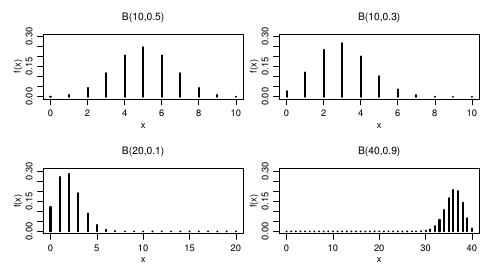
\includegraphics[scale=0.75]{images/binomial_pmf} 
    \caption{Binomial probability mass function}
    \label{fig: binomial pmf}
\end{figure}

\begin{boite}
    \evid{Definition 66.} A \textbf{\textcolor{red}{geometric}} random variable $X$ has PMF 
    \begin{equation}
        f_X(x) =p(1-p)^{x-1} \qquad x=1,2,... \quad 0 \leq p \leq 1
        \label{equ:distribution_geometric}
    \end{equation}
    We write $X \sim Geom(p)$ and call p the \uline{success probability}. 
    \begin{blackbox}
        This models the waiting time until a first event, in a series of independent    trials having the same success probability
    \end{blackbox}
\end{boite}

\begin{boite}
    \evid{Definition 69.} A \textbf{\textcolor{red}{negative binomial}} random variable $X$ with parameters $n$ and $p$ has PMF
    \begin{equation}
        f_X(x) = \combi{x-1}{n-1}p^n(1-p)^{x-n} \qquad x = n, n+1, n+2,... \quad 0 \leq p \leq 1
        \label{equ:distribution_negative_binomial}
    \end{equation}
    We write $X \sim NegBin(n,p)$. With $n=1,\ X \sim Geom(p)$.
    \begin{blackbox}
        It models the waiting time until the $n$\ts{th} success in a series of independent trials having the same success probability
    \end{blackbox}
\end{boite}
\begin{exemple}
    Find the probability of seeing 2 heads before 5 tails in repeated tosses of a coin
\end{exemple}

We can write the geometric and binomial variables in a more general form, setting $Y = X-n$, and using the gamma function :
\[f_Y(y) = \frac{\Gamma(y+\alpha)}{\Gamma(\alpha)y!}p^{\alpha}(1-p)^y,\qquad y =0,1,2,\ldots \quad 0 \leq p \leq 1,\ \alpha > 0\]
Where the \textcolor{red}{gamma function} is :
\begin{equation}
    \Gamma(\alpha) = \int_0^\infty u^{\alpha-1}e^{-u} \deriv{u},\quad \alpha > 0
    \label{equ:gamma_function}
\end{equation}
with some properties :
\begin{multicols}{2}
    \begin{itemize}
        \item $\Gamma(1)$
        \item $\Gamma(\alpha+1) = \alpha\Gamma(\alpha) \quad \alpha > 0$
        \item $\Gamma(n) = (n-1)!,\quad n=1,2,3,\ldots$
        \item $\Gamma(\frac{1}{2}) = \sqrt{\pi}$
    \end{itemize}
\end{multicols}

\begin{boite}
    \evid{Definition 71.} We draw a sample of $m$ balls without replacement from an urn containing $w$ white balls and $b$ black balls. Let $X$ be the number of white balls drawn. Then :
    \begin{equation}
        P(X=x) = \frac{\combi{w}{x}\combi{b}{m-x}}{\combi{w+b}{m}}
        \label{equ:distribution_hypergeometric}
    \end{equation}
    and the distribution of $X$ is \textbf{\textcolor{red}{hypergeometric}}. We write $X \sim HyperGeom(w,b,m)$
\end{boite}
\evid{Definition 74.} A \textcolor{red}{discrete uniform} random variable $X$ has PMF 
\begin{equation}
    f_X(x) = \frac{1}{b-a+1}, \qquad x = a, a+1,\ldots, b\quad a < b \quad a,b \in \Z
    \label{equ:distribution_discrete_uniform}
\end{equation}

\begin{boite}
    \evid{Definition 75.} A \textbf{\textcolor{red}{Poisson}} random variable $X$ has the PMF
    \begin{equation}
        f_X(x) = \frac{\lambda^x}{x!}e^{-\lambda},\qquad x = 0,1,\ldots,\quad \lambda > 0
        \label{equ:distribution_poisson}
    \end{equation}
    and we write $X \sim Pois(\lambda)$.
\end{boite}

\evid{Definition 76.} The \textcolor{red}{cumulative distribution function (CDF)} of a random variable is 
\[F_X(x) = P(X \leq x),\quad x \in \R\]
if $X$ is discrete, we can write :
\[F_X(x) = \sum_{x_i \in D_X:x:i \leq x} P(X = x_i)\]

Let $X$ be a discrete random variable for which $\sum_{x\in D_X} |x|f_X(x) < \infty$, where $D_X$ is the support of $f_X$. The \textbf{\textcolor{red}{expectation}} (or \textcolor{red}{expected value} of \textcolor{red}{mean}) of $X$ is
\begin{equation}
    \E(X) = \sum_{x\in D_X} xP(X=x) = \sum_{x\in D_X} xf_X(x)
    \label{equ:expectation}
\end{equation}

\subsection{Examples}
\evid{Example 65} A multiple choice test contains 20 questions. For each question, you must choose the correct answer amongst 5 possible answers. A pass is obtained with 10 correct answers. A student picks his answers at random. 
\begin{enumerate}
    \item Give the distribution for his number of correct answers
    \item What is the probability that he will pass the test ?
\end{enumerate}
\uline{Answer :} As X is based on independent trials with a same probability $p$ (with $p = 1/5$) and the total number of trials $n$ is fixed ($n = 20$), then it's a Binomial distribution : $X \sim B(20, 0.2)$. The condition is ``10 or more correct answers''. We thus apply the formula :
\[P(X \geq 10) = \sum_{x=10}^{20}0.2^x(1-0.2)^{20-x} = 0.0026\]
This is quite logical ; term by term : the sum is for ``10 or 11 or 12 or ... or 20 right answers''. All of them are correct. The \combi{20}{x} tells : ``for this given amount of right answers, we chose them amongst all answers'' ; that's ``20 chose x''. Once the $x$ right answers have been picked, we need the probability that those $x$ were correct ($0.2^x$) and, even more, that the $20-x$ other are incorrect (because we look each time at \textit{exactly} $x$ right answers). That gives $(1-0.2)^{20-x}$
\subsection{Exercises}


%%%%%%%%%%%%%%%%%%%%%%%%%%%%%%%%%%%%%%%%%%
%%%%%%%%%%%%%%%%%%%%%%%%%%%%%%%%%%%%%%%%%%
%%%%%%%%%%%%%%%%%%%%%%%%%%%%%%%%%%%%%%%%%%
\section{Week 4}
Concerns slides 112-135. Transformations of discrete variables. Expectation, examples and properties. Moments/variance. Conditional distributions and their moments. Convergence and small numbers. Relations among distributions. Start of continuous variables.
\subsection{Theorems and definitions}
\evid{Theorem 87.} Let $X$ be a random variable with mass function $f$ and let $g$ be a real-valued function of \R. Then 
\[E\{g(X)\} = \sum_{X\in D_X} g(x)f(x)\]
\begin{boite}
    \evid{Definition 90.} If $X$ has a PMF $f(x)$ such that $\sum_x |x|^r f(x) < \infty$, then 
    \begin{enumerate}[label=(\alph*)]
        \item the $r$\ts{th} \textcolor{red}{moment} of $X$ is $\E(X^r)$
        \item the $r$\ts{th} \textcolor{red}{central moment} of $X$ is $\E[\{X-\E(X)\}^r]$
        \item the \textcolor{red}{variance} of $X$ is $var(x) = \E\Big[\big\{X-\E(X)\big\}^2\Big]$ (the second central moment)
        \item the \textcolor{red}{standard deviation} of $X$ is defined as $\sqrt{var(X)}$ (non-negative)
        \item the $r$\ts{th} \textcolor{red}{factorial moment} of $X$ is $\E\big\{X(X-1)\ldots(X-r+1)\big\}$
    \end{enumerate}
\end{boite}
\todo{maybe add properties of variance here}

\subsubsection*{Conditional probability distributions}
\evid{Definition 97.} Let $(\Omega, \mathcal{F}, P)$ be a probability space, on which we define a random variable $X$, and let $B \in \mathcal{F}$ with $P(B) > 0$. Then the \textbf{\textcolor{red}{conditional probability mass function}} of $X$ given $B$ is
\[f_X(x|B) = P(X=x|B)=\frac{P(A_x\cap B)}{P(B)}\]
where $A_x = \{\omega \in \Omega : X(\omega) = x\}$

\evid{Theorem 98.} The function $f_X(x|B)$ satisfies 
\[f_X(x|B) \geq 0,\quad \sum_x f_X(x|B) = 1\]
and is thus a well defined mass function.

\subsubsection*{Notions of convergence}
We often want to approximate one distribution by another. The mathematical basis for doing so is the convergence of distributions.

\evid{Definition 103.} Let $\{X_n\}$ be random variables whose cumulative distribution fonctions are $\{F_n\},F$ Then we say that the random variables $\{X_n\}$ \textbf{\textcolor{red}{converge in distribution}} (or \textcolor{red}{converge in law}) to $X$, if for all $x \in \R$, where $F$ is continuous,
\begin{equation}
    F_n(x) \to F(x),\qquad n\to \infty
\end{equation}
We write $X_n \overset{D}{\longrightarrow} X$
\begin{boite}
    \evid{Lemma 104.} $n^{-r} \combi{n}{r} \to \frac{1}{r!}$ for all $r\in \N$, when $n \to \infty$
\end{boite}
\begin{boite}
    \evid{Theorem 105.} \textbf{Law of small numbers :} Let $X_n \sim B(n,p_n)$, and suppose that $np_n \to \lambda > 0$, when $n\to \infty$. Then $X_n \overset{D}{\longrightarrow} X$, where $X \sim Pois(\lambda)$.
\end{boite}
It was not told during the lectures (nor in the slides), but this law seems to be usable only when $n \geq 50$ and $np \leq 5$. 

A summary (flowchart) of the correct use of distributions is to be found at appendix \ref{app:which_distribution}


%%%%%%%%%%%%%%%%%%%%%%%%%%%%%%%%%%%%%%%%%%
%%%%%%%%%%%%%%%%%%%%%%%%%%%%%%%%%%%%%%%%%%
%%%%%%%%%%%%%%%%%%%%%%%%%%%%%%%%%%%%%%%%%%


\section{Week 5}
Concerns slides 136 to 161. Continuous variables: definition,e xamples, moments. Conditional densities and expectation. Quantiles, transformation of scalar variables. Normal distribution, basic properties, use of table $\Phi$
\subsection{Theorems and definitions}
\evid{Definition 111.} A random variable $X$ is \textbf{continuous} if there exists a function $f(x)$, called the \textbf{probability density function (or density) PDF} of $X$, such that 
\begin{equation}
    P(X \leq x) = F(x) = \int_{-\infty}^x f(u) \deriv{u},\quad x \in \R
\end{equation}
\evid{Definition 112} (Uniform distribution) The random variable $U$ having density
\[f(u) = \left\{\begin{array}{ll}
    \frac{1}{b-a} & a \leq u \leq b\\
    0 & \text{Otherwise}
\end{array}\right. \quad a < b\]
is called a \textcolor{red}{uniform random variable}. We write $U \sim U(a,b)$.\\
\evid{Definition 113.} (Exponential distribution). The random variable $X$ having density 
\[f(x) = \left\{\begin{array}{ll}
    \lambda e^{-\lambda x} & x > 0\\
    0 & \text{Otherwise}
\end{array}\right.\]
is called an \textcolor{red}{exponential random variable} with parameter $\lambda > 0$. We write $X \sim \exp(\lambda)$
\uline{In practice}, random variables are almost always either discrete or continuous, with exceptions such as daily rain totals.\\
\evid{Definition 115.} (Gamma distribution) The random variable $X$ having density 
\[f(x) = \left\{\begin{array}{ll}
    \frac{\lambda^\alpha}{\Gamma(\alpha)}x^{\alpha-1}e^{-\lambda x} & x > 0\\
    0 & \text{Otherwise}
\end{array}\right.\]
is called a \textcolor{red}{gamma random variable} with parameters $\alpha, \lambda > 0$ ; we write $X \sim \Gamma(\alpha, \lambda)$. Here, $\alpha$ is called the \textbf{shape parameter} and $\lambda$ is called the \textbf{rate} with $\lambda^{-1}$ the \textbf{scale parameter}. By letting $\alpha = 1$, we get the exponential density, and when $\alpha = 2,3,...$ we get the \textbf{Erlang} density.

\evid{Pareto random variable} The random variable $X$ with cumulative distribution function 
\[F(x) = \left\{\begin{array}{ll}
    0 & x < \beta\\
    1 - \(\frac{\beta}{x}\)^\alpha & x \geq \beta
\end{array}\right.\]
is called a \textcolor{red}{Pareto random variable}

\evid{Expectation of $g(X)$.} Let $g(x)$ be a real-valued function and $X$ a continuous random variable of density $f(x)$. Then if $\E\{|g(xX)|\} < \infty$, we define the \textcolor{red}{expectation of $g(X)$} to be 
\begin{equation}
    \E\{g(X)\} = \int_{-\infty}^{\infty} g(x)f(x) \deriv{x}
\end{equation}
In particular, the expectation and the variance of $X$ are :
\begin{align}
    \E(X) = \int_{-\infty}^{\infty} x f(x) \deriv{x}\\
    var(x) = \int_{-\infty}^{\infty}\{x - \E(X)\}^2 f(x)\deriv{x} = E(X^2) - E(X)^2
\end{align}

\evid{Definition 123.} Let $0 < p <1$. We define the $p$ \textcolor{red}{quantile} of the cumulative distribution function $F(x)$ to be 
\begin{equation}
    x_p = \inf\{x: F(x) \geq p\}
\end{equation}
For most continuous random variables, $x_p$ is unique and equals $x_p = F^{-1}(p)$, where $F^{-1}$ is the inverse function of $F$ ; then $x_p$ is the value for which $P(X \leq x_p) = p$. In particular, we call the $0.5$ quantile the \textcolor{red}{median} of $F$.

\evid{Definition 129.} Let $g: \rtor$ be a function and $B \subset \R$ any subset of \R. Then, $g^{-1}(B) \subset \R$ is the set for which $g\{g^{-1}(b)\} = B$

\evid{Theorem 130.} Let $Y = g(X)$ be a random variable and $B_y  (-\infty, y]$. Then :
\begin{equation}
    F_Y(y) = P(Y \leq y) = 
    \left\{\begin{array}{ll}
        \int_{g^{-1}(B_y)}f_X(x)\deriv{x} & X \text{ continuous}\\
        \sum_{x\in g^{-1} (B_y)}f_X(x) & x \text{ discrete}
    \end{array}\right.
\end{equation}
where $g^{-1}(B_y) = \{x \in \R : g(x) \leq y\}$. When $g$ is monotone increasing or decreasing and has inverse $g^{-1}$, then
\begin{equation}
    f_Y(y) = \left|\frac{\deriv{g^{-1}}(y)}{\deriv{y}}\right| f_X\{g^{-1}(y)\}
\end{equation}

\subsection*{Normal distribution}
\evid{Definition 133.} A random variable $X$ having density
\[f(x)= \frac{1}{(2\pi)^{\frac{1}{2}}\sigma} \exp\left\{-\frac{(x-\mu)^2}{2\sigma^2}\right\}\]
is a \textcolor{red}{normal random variable} with expectation $\mu$ and variance $\sigma^2$ : we write $X \sim \mathcal{N}(\mu, \sigma^2)$. When $\mu = 0, \sigma^2 = 1$, the corresponding random variable $Z$ is \textcolor{red}{standard normal}, $Z \sim \mathcal{N}(0,1)$, with density 
\[\phi(z) = (2\pi)^{-\frac{1}{2}}e^{-\frac{z^2}{2}},\quad z \in \R\]

\evid{Theorem 135.} The density $\phi(z)$, the cumulative distribution $\Phi(z)$ and the quantiles $z_p$ of $Z \sim \mathcal{N}(0,1)$, satisfy for all $z \in \R$ :
\begin{enumerate}[label = (\alph*)]
    \item the density is symmetric with respect to $z = 0$, i.e. $\phi(z) = \phi(-z)$
    \item $P(Z \leq z) = \Phi(z) = 1-\Phi(-z) = 1-P(Z \geq z)$
    \item the standard normal quantiles $z_p$ satisfiy $z_p = -z_{1-p}$, for all $0 < p< 1$
    \item $z^r\phi(z) \to 0$ when $z \to \pm \infty$, for all $r > 0$. This implies that the moments $E(Z^r)$ exists for all $r \in \N$
    \item we have 
            \[\phi'(z) = -z\phi(z),\ \phi''(z) = (z^2 -1)\phi(z),\ \phi'''(z) = -(z^3-3z)\phi(z),\ \ldots\]
    \item If $X \sim \mathcal{N}(\mu, \sigma^2$, then we can write $X = \mu + \sigma Z$, where $Z \sim \mathcal{N}(0,1)$.
\end{enumerate}
\subsection{Examples}
\subsection{Exercises}
%%%%%%%%%%%%%%%%%%%%%%%%%%%%%%%%%%%%%%%%%%
%%%%%%%%%%%%%%%%%%%%%%%%%%%%%%%%%%%%%%%%%%
%%%%%%%%%%%%%%%%%%%%%%%%%%%%%%%%%%%%%%%%%%
\section{Week 6}
\subsection{Theorems and definitions}
\subsubsection*{Several random variables}
\evid{Definition 145.} Let $(X,Y)$ be a discrete random variable: the set 
\[D = \big\{(x,y) \in \R^2 : P(\{(X,Y) = (x,y)\} > 0\big\}\]
is countable. The \textbf{\textcolor{red}{(joint) PMF}} of $(X,Y)$ is 
\[f_{X,Y} = (xmy) = P\{(X,Y) = (x,y)\},\quad (x,y) \in \R^2\]
and the \textbf{\textcolor{red}{(joint) CDF}} of $(X,Y)$ is 
\[F_{X,Y} (x,y) = P(X \leq x, Y \leq y),\quad (x,y) \in \R^2\]

\evid{Definition 147.} the random variable $(X,Y)$ is said to be \textcolor{red}{(jointly) continuous} if there exists a function $f_{X,Y}(x,y)$ called the \textcolor{red}{(joint) density} of $(X,Y)$ such that 
\[P\big\{(X,Y) \in A\big\} = \iint_{(u,v) \in A} f_{X,Y}(u,v) \deriv{u}\deriv{v}\quad (x,y) \in \R^2\]
By letting $\mathcal{A} = \big\{(u,v) : u \leq x,\ v \leq y\big\}$, we see that the \textcolor{red}{(joint) CDF} of $(X,Y)$ can be written 
\[F_{X,Y}(x,y) = P(X \leq x, Y \leq y) = \int_{-\infty}^{x}\int_{-\infty}^{y}f_{X,Y}(u,v) \deriv{u}\deriv{v} \quad (x,y) \in \R^2\]
and this implies that 
\begin{equation}
    f_{X,Y}(x,y) = \frac{\partial^2}{\partial x \partial y}F_{X,Y}(x,y)
\end{equation}

\evid{Definition 149.} The \textbf{\textcolor{red}{marginal probability mass/density function}} of $X$ is 
\[f_X(x) = \left\{
    \begin{array}{ll}
        \sum_y f_{X,Y}(x,y) & \text{discrete case}\\
        \int_{-\infty}^{\infty} f_{X,Y}(x,y) \deriv{y} & \text{continuous case}
    \end{array}\right. \quad x \in \R\]
and the \textbf{\textcolor{red}{conditional probability mass/density function}} of $Y$ given $X$ is :
\begin{equation}
    f_{Y|X}(y|x) = \frac{f_{X,Y}(x,y)}{f_X(x)}
\end{equation}

It is possible to extrapolate to several variables :\\
\evid{Definition 153.} Let $X_1,\ldots,X_n$ be rvs defined on the same probability space. Their \textcolor{red}{joint CDF} is 
\[F_{X_1,\ldots,X_n}(x_1,\ldots,x_n) = P(X_1 \leq x_1,\ldots,X_n \leq x_n)\]
and their \textcolor{red}{joint density/mass probability function} is :
\[F_{X_1,\ldots,X_n}(x_1,\ldots,x_n) = \left\{\begin{array}{ll}
    P(X_1=x_1,\ldots, X_n = x_n) & \text{discrete case}\\
    \frac{\partial^n F_{X_1,\ldots,X_n}(x_1,\ldots,x_n)}{\partial x_1\ldots \partial x_n} & \text{continuous case}
\end{array}
\right.\]

\evid{Definition 156.} Random variable $X,Y$ defined on the same probability space are \textcolor{red}{independent} if 
\[P(X \in \mathcal{A}, Y \in \mathcal{B}) = P(X \in \mathcal{A})P(Y \in \mathcal{B})\]

\evid{Definition 161.} Let $X,Y$ be random variables of density $f_{X,Y}(x,y)$. The if $\E\{|g(X,Y)|\} < \infty$, we can define the \textcolor{red}{expectation} of $g(X,Y)$ to be  \todo{}

\evid{Definition 166.} The \textbf{\textcolor{red}{correlation}} of $X,Y$ is 
\begin{equation}
    corr(X,Y) = \frac{cov(X,Y)}{\sqrt{var(X)var(Y)}}
\end{equation}

\subsection{Examples}
\subsection{Exercises}
%%%%%%%%%%%%%%%%%%%%%%%%%%%%%%%%%%%%%%%%%%
%%%%%%%%%%%%%%%%%%%%%%%%%%%%%%%%%%%%%%%%%%
%%%%%%%%%%%%%%%%%%%%%%%%%%%%%%%%%%%%%%%%%%
\section{Week 7}
\subsection{Theorems and definitions}
\subsection{Examples}
\subsection{Exercises}
%%%%%%%%%%%%%%%%%%%%%%%%%%%%%%%%%%%%%%%%%%
%%%%%%%%%%%%%%%%%%%%%%%%%%%%%%%%%%%%%%%%%%
%%%%%%%%%%%%%%%%%%%%%%%%%%%%%%%%%%%%%%%%%%
\section{Week 8}
\subsection{Theorems and definitions}
\subsection{Examples}
\subsection{Exercises}
%%%%%%%%%%%%%%%%%%%%%%%%%%%%%%%%%%%%%%%%%%
%%%%%%%%%%%%%%%%%%%%%%%%%%%%%%%%%%%%%%%%%%
%%%%%%%%%%%%%%%%%%%%%%%%%%%%%%%%%%%%%%%%%%
\section{Week 9}
\subsection{Theorems and definitions}
\subsection{Examples}
\subsection{Exercises}
%%%%%%%%%%%%%%%%%%%%%%%%%%%%%%%%%%%%%%%%%%
%%%%%%%%%%%%%%%%%%%%%%%%%%%%%%%%%%%%%%%%%%
%%%%%%%%%%%%%%%%%%%%%%%%%%%%%%%%%%%%%%%%%%
\section{Week 10}
\subsection{Theorems and definitions}
\subsection{Examples}
\subsection{Exercises}
%%%%%%%%%%%%%%%%%%%%%%%%%%%%%%%%%%%%%%%%%%
%%%%%%%%%%%%%%%%%%%%%%%%%%%%%%%%%%%%%%%%%%
%%%%%%%%%%%%%%%%%%%%%%%%%%%%%%%%%%%%%%%%%%
\section{Week 11}
\subsection{Theorems and definitions}
\subsection{Examples}
\subsection{Exercises}
%%%%%%%%%%%%%%%%%%%%%%%%%%%%%%%%%%%%%%%%%%
%%%%%%%%%%%%%%%%%%%%%%%%%%%%%%%%%%%%%%%%%%
%%%%%%%%%%%%%%%%%%%%%%%%%%%%%%%%%%%%%%%%%%
\section{Week 12}
\subsection{Theorems and definitions}
\subsection{Examples}
\subsection{Exercises}
%%%%%%%%%%%%%%%%%%%%%%%%%%%%%%%%%%%%%%%%%%
%%%%%%%%%%%%%%%%%%%%%%%%%%%%%%%%%%%%%%%%%%
%%%%%%%%%%%%%%%%%%%%%%%%%%%%%%%%%%%%%%%%%%
\section{Week 13}
\subsection{Theorems and definitions}
eom
\subsection{Examples}
grsg
\subsection{Exercises}
grg




\appendix
\section{Some useful tips}
\subsection{Which distribution ?}
\label{app:which_distribution}
Is $X$ based on independent trials (0/1) with a same probability $p$, or on draws from a finite population with replacement ?
\begin{itemize}
    \item     If \textbf{Yes}, is the total number of trials $n$ fixed, so $X \in \{0,...,n\}$
              \begin{itemize}
                  \item if \textbf{Yes} : use the \textbf{binomial} distribution \ref{equ:distribution_binomial} , $X \sim B(n,p)$ (and thus the \textbf{Bernoulli} distribution if $n = 1$\\
                        $\to$ if $n \simeq \infty$ or $n \gg p$, we can use the \textbf{Poisson} distribution, $X \sim Pois(np)$
                  \item if \textbf{No}, then $X \in \{n, n+1, \ldots\}$, and we use the \textbf{geometric} (if $X$ is the number of trials until ons success) or \textbf{negative binomial} (if $X$ is the number of trials until the last of several successes) distributions.
              \end{itemize} 
    \item     If \textbf{No}, then if the draws is independent but without replacement from a finite population, then
    $X \sim$ \textbf{Hypergeometric} distribution.
\end{itemize}
With a reminder of distributions : 
\begin{itemize}
    \item \textbf{\textcolor{red}{binomial}} random variable  ($X \sim B(n,p)$) ; $n =1 \iff$ Bernoulli trial.
            \begin{equation*}
                f(x) = \combi{n}{x} p^x(1-p)^{n-x},\quad x = 0,1,..,n,\quad n \in \N,\ 0\leq p \leq 1
            \end{equation*}
            Number of successes in a fixed number of trials (indep. of same prob.). It's expected value is $np$ and variance is $np(1-p)$
    \item \textbf{\textcolor{red}{geometric}} random variable ($X \sim Geom(p)$)
            \begin{equation}
                f_X(x) =p(1-p)^{x-1} \qquad x=1,2,... \quad 0 \leq p \leq 1
            \end{equation}
            Waiting time in a series of indep. trials having the same success prob. It's expected value is $\frac{1}{p}$ and variance is $\frac{1-p}{p^2}$
    \item \textbf{\textcolor{red}{negative binomial}} random variable ($X \sim NegBin(n,p)$) ; $n=1 \iff X \sim Geom(p)$.
            \begin{equation}
                f_X(x) = \combi{x-1}{n-1}p^n(1-p)^{x-n} \qquad x = n, n+1, n+2,... \quad 0 \leq p \leq 1
                \label{equ:distribution_negative_binomial}
            \end{equation}
            Waiting time until $n\ts{th}$ success happens (independent, same prob. trials)
   \item \textbf{\textcolor{red}{hypergeometric}} : Sample of $m$ balls without replacement, total of $w$ white balls and $b$ black balls. Let $X$ be the number of white balls drawn ; $X \sim HyperGeom(w,b,m)$
            \begin{equation}
                P(X=x) = \frac{\combi{w}{x}\combi{b}{m-x}}{\combi{w+b}{m}}
            \end{equation}
            It has an expected value of $m\frac{w}{w+b}$
    \item \textbf{\textcolor{red}{Poisson}} random variable ($X \sim Pois(\lambda)$)
    \begin{equation}
        f_X(x) = \frac{\lambda^x}{x!}e^{-\lambda},\qquad x = 0,1,\ldots,\quad \lambda > 0
    \end{equation}
    $E(x) = var(x) = \lambda$ (proof slides 115 and 118)
\end{itemize}


\section{Glossary of functions}
\begin{itemize}
    \item Binomial coefficient :
            \begin{equation}
                \combi{n}{k} = \frac{n!}{k!(n-k)!} = C_n^k
            \end{equation}
    \item 
\end{itemize}

\section{Properties}
\begin{itemize}
    \item For binomial coefficients :
            \begin{itemize}
                \item $\combi{n}{r} = \combi{n}{n-r}$
                \item $\combi{n+1}{r} = \combi{n}{r-1} + \combi{n}{r}$
                \item $\sum_{j=0}^{r}\combi{m}{j}\combi{n}{r-j} = \combi{m+n}{r}$
\end{itemize}
\end{itemize}



\end{document} 